\documentclass[12pt,a4paper]{article}
\usepackage[utf8]{inputenc}
\usepackage[ngerman]{babel}
\usepackage[T1]{fontenc}
\usepackage{amsmath}
\usepackage{amsfonts}
\usepackage{amssymb}
\usepackage{graphicx}
\usepackage{subfigure}
\author{Manuel Mende}
\title{Evaluation des genetischen Algorithmus}
\begin{document}
\maketitle
\section{Manuell erzeugte Testfälle}
Um die vom genetischen Algorithmus erzeugten Testfälle bewerten zu können, werden Testfälle zum Vergleich benötigt. Einige sinnvolle Testfälle werden in Tabelle \ref{tab:testfaelle} präsentiert.
\begin{table}\centering
\begin{tabular}{l|l|l|l|l}
Position & Winkel & Parklücke & Fitness & Reale Eignung \\\hline
5/0 & 0 & 2.5/1 & $0.0$ & Kollision \\\hline
-5/0 & 0 & 2.5/1 & $0.0$ & Kollision \\\hline
4/0 & 0 & 2.5/1 & $0.039828$ & Beinahe Kollision\\\hline
-4/0 & 0 & 2.5/1 & $0.039828$ & Beinahe Kollision\\\hline
2/0 & 270 & 2.5/1 & $0.0$ & Kollision \\\hline
2.5/0 & 180 & 5/2 & $0.0$ & Falsches Ziel und Kollision \\\hline
-2.5/0 & 180 & 5/2 & $0.008106$ & Falsches Ziel \\
\end{tabular}
\caption{Manuell gewählte Testfälle}
\label{tab:testfaelle}
\end{table}
Die ersten zwei Testfälle starten sehr weit außen. Sie führen zur Kollision mit einem Hindernis, dennoch ist die Fitness der Chromosome schlecht. Die zweiten Testfälle starten etwas näher an der Parklücke. Die Fahrspur führt eng an den Rändern der engen Parklücke vorbei, es ergibt sich ein entsprechend hoher Fitnesswert. Der fünfte Fall startet direkt Richtung Wand. Dadurch bedingt kommt es zur Kollision. Auch hier ist der Fitnesswert gering. Fall sechs und sieben starten, als wäre die Parklücke auf der linken Seite -- also um 180 Grad gedreht. Die hier abgefahrene Spur ist überflüssig Komplex. Der Parkassistent versucht ein Rechtsszenario zu realisieren. Im ersten Fall kommt es sogar zur Kollision, trotz riesiger Parklücke. Dennoch ist die Fitness sehr klein.
\begin{figure}\centering
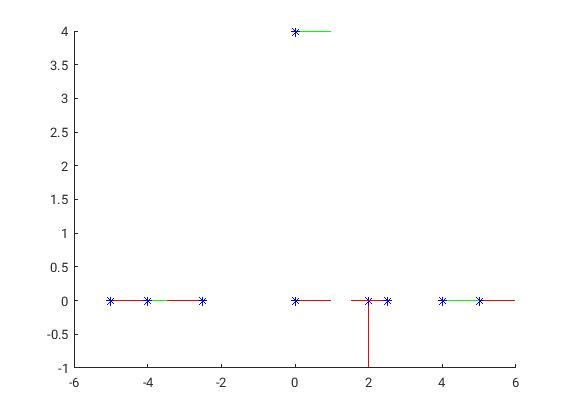
\includegraphics[width=.6\textwidth]{myTestcases.jpg}
\caption{Visualisierung der Testfälle}
\label{fig:testcases}
\end{figure}
Abbildung \ref{fig:testcases} zeigt die Gesamtheit der manuell ausgewählten Testfälle.

\section{Automatisch erzeugte Testfälle}
Der genetische Algorithmus erzeugt Testfälle. Um die Güte der Testfälle beurteilen zu können, sollen zwei Dimensionen analysiert werden. Zum einen wie sinnvoll die ermittelten Testfälle sind und zum anderen wie deterministisch die Ermittlung abläuft.

\subsection{Konvergenz und statistisches Verhalten}
Sinnvoll ist für das Konvergenz-verhalten zu analysieren, wie stark sich der Fitnesswert durch mehr Generationen verbessert.
Dazu wird die Anzahl simulierter Epochen Schrittweise erhöht. Abbildung \ref{fig:epochen} zeigt einen aufgezeichneten Simulationsverlauf. Die Generationen wurden in Zehnerschritten erhöht und der Mittelwert über alle Chromosome der Endgeneration verglichen.
\begin{figure}\centering
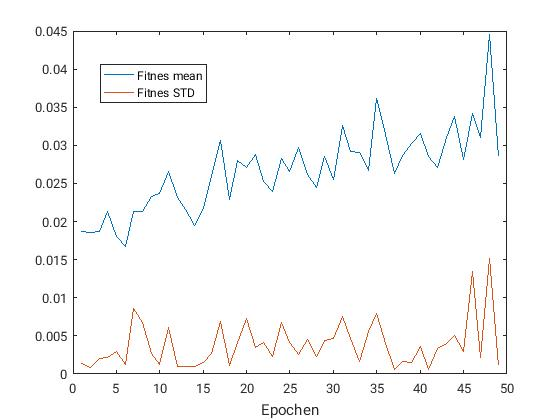
\includegraphics[width=.6\textwidth]{increasedEpochs.jpg}
\caption{Entwicklung der Fitness}
\label{fig:epochen}
\end{figure}
Es kann eine steigende Tendenz festgestellt werden. Je mehr Generationen simuliert werden, desto höher ist der resultierende Wert der Gesamt-Fitness.

\subsection{Äquivalenzklassen}
Äquivalenzklassen erlauben es, Aussagen über die Ähnlichkeit von Testfällen zu machen. Die Tabelle \ref{tab:avgTestfaelle} listet die Mittelwerte sowie Standardabweichungen für 100 Chromosome die über die gegebene Anzahl an Epochen durch Evolution ermittelt wurden.
\begin{table}\centering
\subfigure{
\begin{tabular}{l|l|l}
50 Epochen & Mittelwert & Abweichung \\\hline
X-Position & 0.515882 & 2.301561 \\
Y-Position & 0.888431 & 0.934355 \\
Orientation & 2.456849 & 2.272890 \\
Slot-Length & 2.402382 & 0.164123 \\
Slot-Depth & 1.158000& 0.125341 
\end{tabular}}
\subfigure{
\begin{tabular}{l|l|l}
500 Epochen  & Mittelwert & Abweichung \\
\hline
X-Position & 0.352941&	2.883735\\
Y-Position  & -0.538824&	0.420933\\
Orientation &  3.691803&	2.331866\\
Slot-Length & 2.308667	&0.092787\\
Slot-Depth  & 1.116588	&0.148013\\
\end{tabular}}
\caption{Gemittelte Testfälle}
\label{tab:avgTestfaelle}
\end{table}
\begin{figure}\centering
\subfigure[0 Epochen]{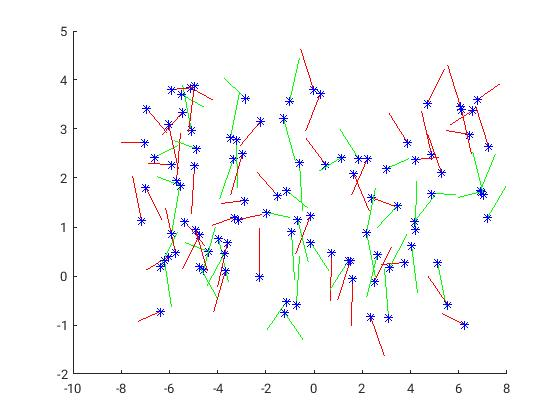
\includegraphics[width=.48\textwidth]{initialTCs.jpg}\label{fig:epochen0}}
\subfigure[500 Epochen]{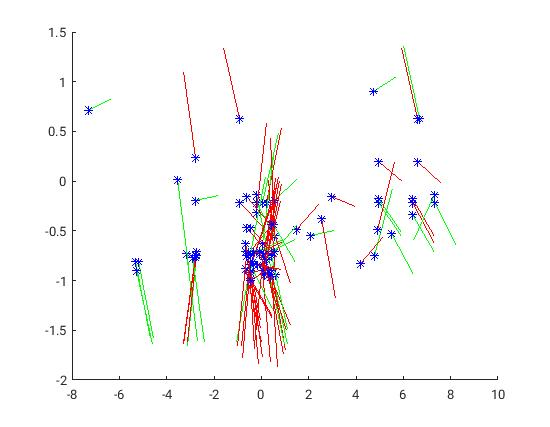
\includegraphics[width=.48\textwidth]{testcases_100chr_500epochs.jpg}\label{fig:epochen500}}
\caption{100 Chromosome}
\label{fig:realTCs}
\end{figure}
Es lässt sich eine Tendenz zu kleinen Parklücken feststellen, vor allem die Länge der Parklücke wird über die Epochen reduziert. Auch die Abweichung ist gering. Die Position des Fahrzeugs streut in x-Richtung sehr stark, das gleiche gilt für die Orientierung des Fahrzeugs. Die y-Position des Fahrzeugs stellt sich auf negative Werte ein, auch hier ist eine Tendenz erkennbar. Abbildung \ref{fig:realTCs} zeigt 100 Testfälle, die durch den genetischen Algorithmus ermittelt wurden. Wieder zeigen Rote Testfälle eine hohe Fitness, und grüne Testfälle eine Vergleichsweise geringe Fitness an. Abbildung \ref{fig:epochen500} stellt die resultierenden Testfälle nach 100 Generationen dar. Dabei wird die größe der Parklücke ausgenommen. Es wird deutlich, dass die Testfälle stark dazu tendieren, das Fahrzeug in der Mitte der Parklücke starten zu lassen. Die Orientierung spielt eine untergeordnete Rolle. Besonders beim Vergleich mit der zufälligen Initialbelegung in Abbildung \ref{fig:epochen0}.

\section{Güte der automatischen Testfälle}
Zum Abschluss müssen die gefundene Testfälle beurteilt werden. Der Algorithmus scheint zu einer speziellen Art Testfälle -- zentral zur Parklücke -- zu tendieren. Die manuell ermittelten Testfälle sind anders strukturiert. Dennoch sind die Ergebnisse zufriedenstellen. Sie ergeben eine Tendenz, dass es Hilfreich ist, das Fahrzeug schon teilweise in der Parklücke starten zu lassen. Andererseits werden viele interessante Testfälle nicht gefunden. Im besonderen sollten Linksparkszenarien untersucht werden, da hier der Parkvorgang wesentlich effizienter und robuster gestaltet werden kann. Dies würde eine Modifikation der Fitness-Funktion voraussetzen. Auch werden Kollisionen stiefmütterlich behandelt. Zwar sind einige Szenarien sicherlich auszuklammern, weil sie die Systemgrenzen übersteigen -- wie direkt Richtung Wand zu starten. Aber es kann auch bei weiten Strecken und engen Lücken zu Kollisionen kommen. Diese Testfälle werden unterbewusst unterdrückt.

\end{document}